% sections/arm_reset.tex: the adjustable-rate reset design in the bureau (E12, E12b, I10, I10b; exhibits from Code/exhibits/make_arm_figures.R).
\subsection{First Mortgages: Adjustable-Rate Resets as a Rule-Based Experiment}\label{sec:armreset}

\paragraph{The design in summary.} Hybrid adjustable-rate mortgages originated in 2004 to 2008 reset to an index rate at a date fixed at origination, 36, 60 or 84 months after opening, and for resets in 2010 to 2013 the payment fell at a known date by an amount set by the initial rate and the index, with the balance unchanged. The panel has no contract flag. The amortization identity recovers the note rate from the balance path and separates a rate reset from an escrow re-analysis, and among 429,078 payment changes on the 1,585,852 first mortgages of those vintages it finds 6,348 rate cuts at the hybrid reset ages, with the implied note rate falling from 6.0 to 3.2 percent at the median (Table \ref{tab:arm_classes}). No rate is obtained from them, for three reasons the data establish. The one-year Treasury rate moved by less than 0.2 percentage points across the four reset years while the resets moved note rates by 2.4 points, so the size of a reset has no source of variation outside the borrower's own initial rate, which is priced on her risk, and the instrument built from the index has a first-stage $F$ statistic below two in every sample. In the four months before a cut, delinquency is higher before a larger coming cut: the coefficient on the coming log change is $-0.47$ (standard error $0.13$) against $-0.50$ ($0.36$) at the change (Table \ref{tab:arm_samples}), and under Proposition \ref{prop:sensT} the response $\tau$ months before a known change is $D(\tau)Q_\tau\lambda$ times the response at it and has its sign under every discount function, every survival process and every present-payment premium, so the profile is generated by a process outside the borrower's valuation of the coming payment. And the clean cuts hold 1,066 first 90-day delinquency events, so the standard error at the change is twice the coefficient the panel's own payment elasticity implies. What the resets establish is the method that finds them without a contract flag and the sign of the pre-reset process; Appendix \ref{appendix:timing} reports the classification of every payment change, the event study and the anticipation profile.

The variation that identifies a discount rate is a payment that changes at a date known in advance, at a fixed balance, for a reason unrelated to the borrower (Proposition \ref{prop:sensT}). Hybrid adjustable-rate mortgages originated in 2004 to 2008, the contracts studied by \citet{fuster_payment_2017}, \citet{keys_mortgage_2014} and \citet{dimaggio_interest_2017}, reset to an index rate at a date fixed at origination, 36, 60 or 84 months after opening, and for resets in 2010 to 2013 the index was far below the initial rate, so the payment fell at a known date by an amount set by the initial rate and the index, with the balance unchanged. This subsection reports what the credit-bureau panel can and cannot measure from those resets. It can measure them: the panel has no contract flag, and the amortization identity recovers the note rate from the balance path, so a rate reset is distinguished from every other reason a mortgage payment changes. It cannot deliver the discount function from them, for three reasons that the data establish rather than suggest: the index did not move across the reset years, so the size of a reset has no source of variation outside the borrower's own contract; delinquency rises in the months before a larger cut in every sample, which no discount function produces; and the one-percent panel holds too few delinquency events on the clean resets to measure the anticipation ratios of Proposition \ref{prop:sensT} at a useful precision.

\paragraph{Finding the resets.} Among the 1,585,852 first mortgages in the panel originated in 2004 to 2008, 429,078 loan-months show a change in the scheduled payment of more than five percent while the balance continues to amortize. A payment change is not a rate change: the scheduled payment reported to the bureau includes the escrow for taxes and insurance, which servicers re-analyze on the loan's anniversary, and the anniversary months coincide with the reset months. The balance path separates the two. With remaining term $n$, balance $B$ and a monthly principal reduction $\pi$, the annuity identity $\pi/B=(r/12)/\big((1+r/12)^{n}-1\big)$ gives the note rate $r$, and the principal-and-interest payment then follows, so that the escrow is the remainder of the reported payment. A rate reset moves the implied rate and leaves the escrow unchanged; an escrow re-analysis moves the escrow and leaves the implied rate within 0.2 percentage points. Table \ref{tab:arm_classes} classifies every payment change by the balance path over the eight months on either side. At the hybrid reset ages, 6,348 cuts are rate changes, with the implied note rate falling from 6.0 to 3.2 percent at the median, the signature of a 2004--08 hybrid resetting to the 2010--13 index; 11,760 changes at those ages are escrow re-analyses of both signs and a median size of ninety dollars; and 27,428 more are interest-only loans, whose balance identifies no rate, recasts, negative amortization, and trades that close within three months of the change, which are transfers and modifications. One payment change in ten at the reset ages is a rate change, and one in fourteen is a rate cut.

\paragraph{What the resets show.} Table \ref{tab:arm_samples} reports, for five samples, the response of first 90-day delinquency to the log change in the payment at and after the change, and the mean response in the four months before it, with loan and vintage-band-by-calendar-month fixed effects, so that the comparison is between loans of the same origination half-year in the same month. Figure \ref{fig:arm_event} shows the hazard around the cuts, and Figure \ref{fig:arm_anticipation} the response at each horizon before the change. On the sample of rate cuts whose balance amortizes before the change, with no condition on the balance after it, the response at the change is $-0.50$ (standard error $0.36$) per unit of log payment, times one hundred: a cut of the median size, 25 percent of the payment, moves a monthly hazard of 0.42 percent by an amount whose 95 percent interval runs from $-0.06$ to $+0.35$ percentage points and includes the $-0.05$ that the panel's payment elasticity of $0.45$ implies. The response is not measured as different from zero or from the panel's payment elasticity. Figure \ref{fig:arm_event} shows why the raw hazard nonetheless falls by a third after the largest cuts: the largest cuts reset in 2010 and 2011, when every vintage's hazard was falling, and the calendar effects remove that fall. The sample that also requires the balance to amortize after the change gives a response of $+0.37$ ($0.16$), an elasticity of $1.3$, but that condition selects on the outcome, because a loan that stops paying at the reset does not amortize afterward, and the response is the selection.

The anticipation profile has the wrong sign in every sample. In the four months before a cut the coefficient on the coming log change is $-0.47$ ($0.13$) on the pre-conditioned sample and $-2.36$ ($0.49$) on the post-conditioned one: delinquency is higher before a larger coming cut, relative to the same loan a year to two years earlier, and the excess is concentrated in the last four months. Proposition \ref{prop:sensT} gives the response $\tau$ months before a known payment change as $D(\tau)\,Q_\tau\,\lambda$ times the response at the change, with $D\in(0,1]$, $Q_\tau\in(0,1]$ and $\lambda>0$. The anticipation response therefore has the sign of the response at the change under every discount function, every survival process and every present-payment premium; a profile of the opposite sign is generated by a process outside the borrower's valuation of the coming payment, and the ratio of the two responses is not $D(\tau)Q_\tau\lambda$ for any $\rho$. Appendix \ref{appendix:strategies} lists this with the other objects that do not identify the rate. Payment rises show the opposite pattern, a response at the change of $3.17$ ($0.40$) and a profile before it that is flat at four tenths of that response over twelve months, and the rises are not certified either: the scheduled-payment field rises when arrears are added to it, so a rise in the reported payment follows delinquency as often as it precedes it.

\paragraph{Why the design cannot be rescued in this period.} The size of a hybrid reset is the difference between the initial rate and the index plus the margin at the reset month. The one-year Treasury rate at the reset months was 0.29 percent at the median in 2010 and 0.13 percent in 2013, so across the four reset years the index moved by less than 0.2 percentage points while the resets moved rates by 2.4 points. The instrument built from the index, the change in the rate between origination and reset within a vintage band, has a first-stage $F$ statistic below two in every sample: there is no variation in the size of a reset in this period that does not come from the borrower's own initial rate, and the initial rate is priced on the borrower's risk. The remaining limit is precision. The clean cuts hold 1,066 first 90-day delinquency events, and the standard error on the response at the change, $0.36$, is twice the coefficient that the panel's own elasticity implies, $0.19$; at each horizon before the change the ratio of the two responses has a standard error near one. The ten-percent archive holds ten times the loans and is observed twice a year, which does not resolve a monthly anticipation profile. The reset design in the bureau therefore establishes the method that finds resets without a contract flag and the sign of the pre-reset process; the discount function has to come from a payment change whose size varies for a reason outside the contract and whose events number in the tens of thousands. The student-loan payment resumption of October 2023, a payment increase on another account at a date fixed by statute four months in advance and of a size fixed by the student loan, is that design, and Appendix \ref{sec:studentloan} reports it.

\begin{table}[H]
\centering
\caption{Payment changes on 2004--08 first mortgages, classified by the balance path}
\label{tab:arm_classes}
\small
\resizebox{\textwidth}{!}{\begin{tabular}{lrrrr}
\toprule
 & \multicolumn{2}{c}{All ages} & \multicolumn{2}{c}{Hybrid reset ages} \\
\cmidrule(lr){2-3}\cmidrule(lr){4-5}
Class of payment change & Down & Up & Down & Up \\
\midrule
Rate change (amortisation before and after) & 16,914 & 22,875 & 6,348 & 2,876 \\
Escrow re-analysis (rate unchanged) & 23,674 & 32,827 & 5,730 & 6,030 \\
Interest-only before and after & 17,028 & 19,313 & 6,285 & 4,427 \\
Interest-only recast & 7,995 & 11,262 & 3,856 & 3,602 \\
Negative amortisation & 9,086 & 8,025 & 2,012 & 1,468 \\
Trade closes within three months & 10,528 & 11,125 & 3,240 & 2,538 \\
Balance path unobserved & 6,119 & 6,523 & 2,630 & 2,095 \\
Unclassified & 60,880 & 76,753 & 18,210 & 16,804 \\
\midrule
Implied note rate, hybrid-age rate changes: before, after (percent) & & & 6.0, 3.2 & 3.9, 6.6 \\
\bottomrule
\end{tabular}
}
\vspace{0.5em}
\begin{minipage}{0.92\textwidth}
\noindent \small \textit{Notes:} Changes in the scheduled payment of more than five percent at an amortizing balance, one-percent panel (monthly archives from 2010), first mortgages originated 2004--08, observed 2005--18. Hybrid reset ages are loan ages within three months of 36, 60 or 84. A rate change is a change in the implied note rate of more than one percentage point in the direction of the payment change that accounts for at least half of it; an escrow re-analysis is an implied-rate change within half a point with the escrow accounting for at least half of the payment change.
\end{minipage}
% replication: Code/extract/E12_arm_paths.R, E12b_arm_implied_rates.R
\end{table}

\begin{figure}[H]
\centering
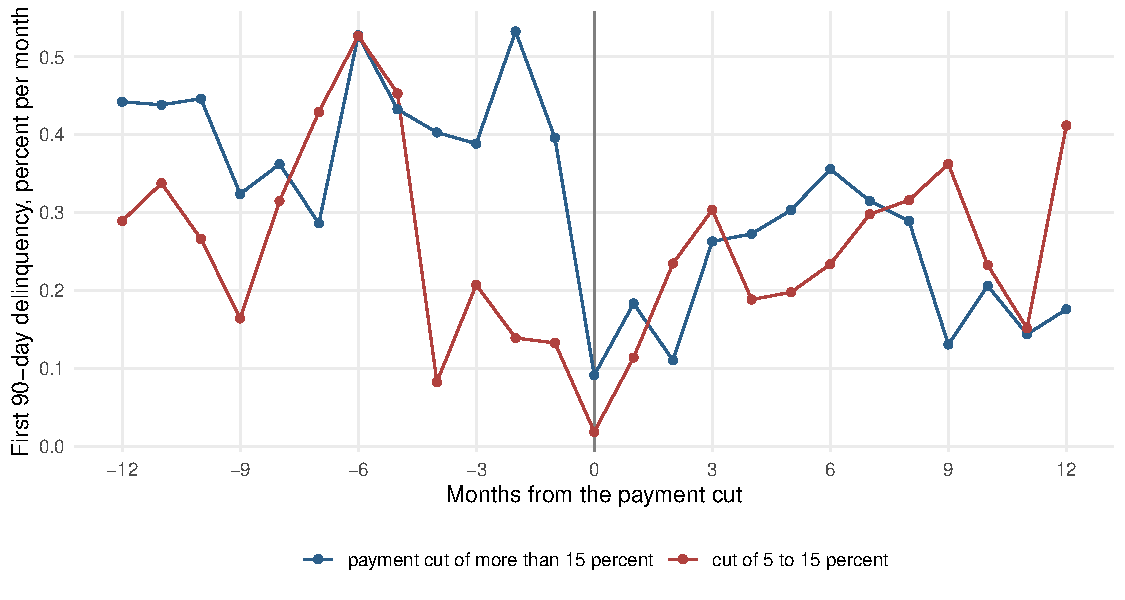
\includegraphics[width=0.85\textwidth]{figures/fig_arm_event.pdf}
\caption{First 90-day delinquency around a payment cut on a mortgage whose balance amortizes before the cut, by the size of the cut. The largest cuts reset in 2010 and 2011; the fall after month three is the calendar decline in delinquency, which the fixed effects of Table \ref{tab:arm_samples} remove.}
\label{fig:arm_event}
% replication: Code/identification/I10_arm_reset.R, Code/exhibits/make_arm_figures.R
\end{figure}

\begin{figure}[H]
\centering
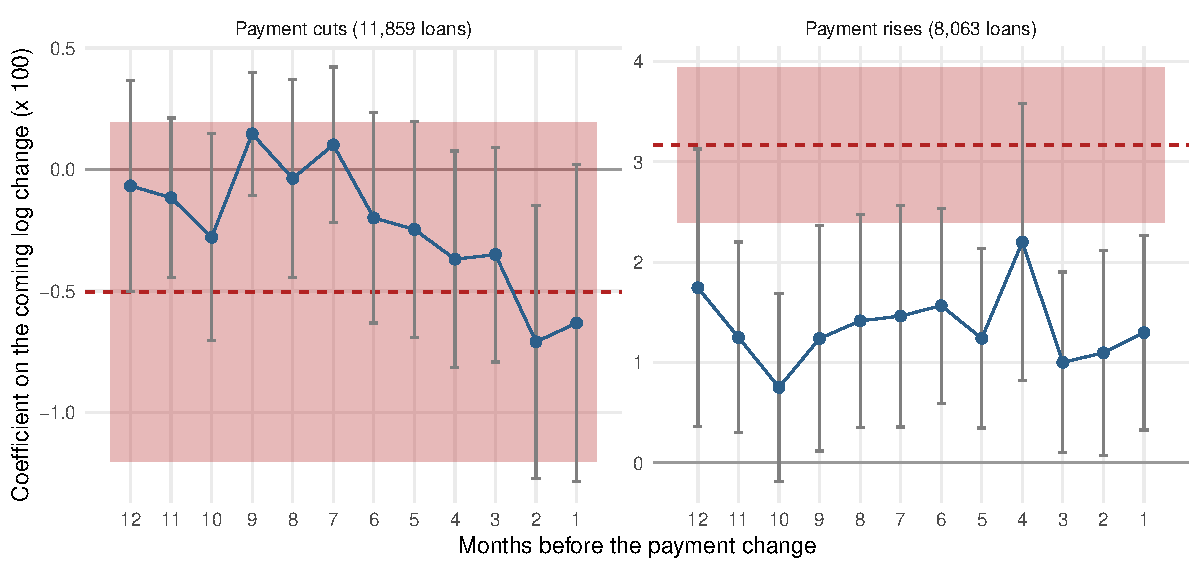
\includegraphics[width=0.95\textwidth]{figures/fig_arm_anticipation.pdf}
\caption{The response of first 90-day delinquency to the coming log payment change at each of the twelve months before it, relative to the same loan 13 to 24 months before, with 95 percent bands; the dashed line and band are the response at the change. Left: rate cuts; right: rate rises. Under Proposition \ref{prop:sensT} the response before the change has the sign of the response at it.}
\label{fig:arm_anticipation}
% replication: Code/identification/I10_arm_reset.R, Code/exhibits/make_arm_figures.R; results/arm_event_study_cut.csv, results/arm_event_classes_detail.csv
\end{figure}

\begin{table}[H]
\centering
\caption{The reset responses across samples}
\label{tab:arm_samples}
\small
\resizebox{\textwidth}{!}{\begin{tabular}{lrrrrr}
\toprule
Sample & Loans & Events & Base hazard & At the change & Before (1--4 months) \\
\midrule
All hybrid-age payment changes & 72,720 & 12,165 & 0.94 & 1.15 (0.08) & -0.99 (0.14) \\
Payment cuts of more than 15 percent & 14,101 & 2,578 & 1.36 & 0.12 (0.08) & -1.19 (0.24) \\
Rate cuts, amortising before and after & 6,114 & 361 & 0.29 & 0.37 (0.16) & -2.36 (0.49) \\
Rate cuts, amortising before & 11,859 & 1,066 & 0.42 & -0.50 (0.36) & -0.47 (0.13) \\
Rate rises, amortising before & 8,063 & 1,218 & 0.54 & 3.17 (0.40) & 1.27 (0.26) \\
\bottomrule
\end{tabular}
}
\vspace{0.5em}
\begin{minipage}{0.92\textwidth}
\noindent \small \textit{Notes:} Linear probability coefficients ($\times 100$) of first 90-day delinquency on the log payment change interacted with an indicator for months at or after the change, and the precision-weighted mean of the coefficients on the coming change at one to four months before it, with loan and origination-half-year-by-calendar-month fixed effects; standard errors clustered by lender-year. Base hazard: percent per month, 13 to 24 months before the change. Samples: all payment changes at hybrid reset ages; cuts of more than 15 percent; rate cuts of Table \ref{tab:arm_classes} with the balance amortizing before and after the cut; rate cuts with the balance amortizing before the cut and the trade open three months after it; rate rises on the same condition.
\end{minipage}
% replication: Code/identification/I10b_arm_reset_iv.R
\end{table}
